%! suppress = MissingImport
%! Author = maxwe
%! Date = 10.03.22

% Preamble
\documentclass[11pt]{PyRollDocs}

\addbibresource{refs.bib}

\newmintinline[py]{python}{}

% Document
\begin{document}

    \title{The Pillar Model PyRoll Plugin}
    \author{Max Weiner}
    \date{\today}

    \maketitle

    The Pillar Model plugin serves as a base package for other plugins using the division of the profile in collinear pillars along width direction.
    It is mainly intended for calculation of material flow, groove filling and spread.


    \section{Model approach}\label{sec:model-approach}

    \begin{figure}
        \centering
        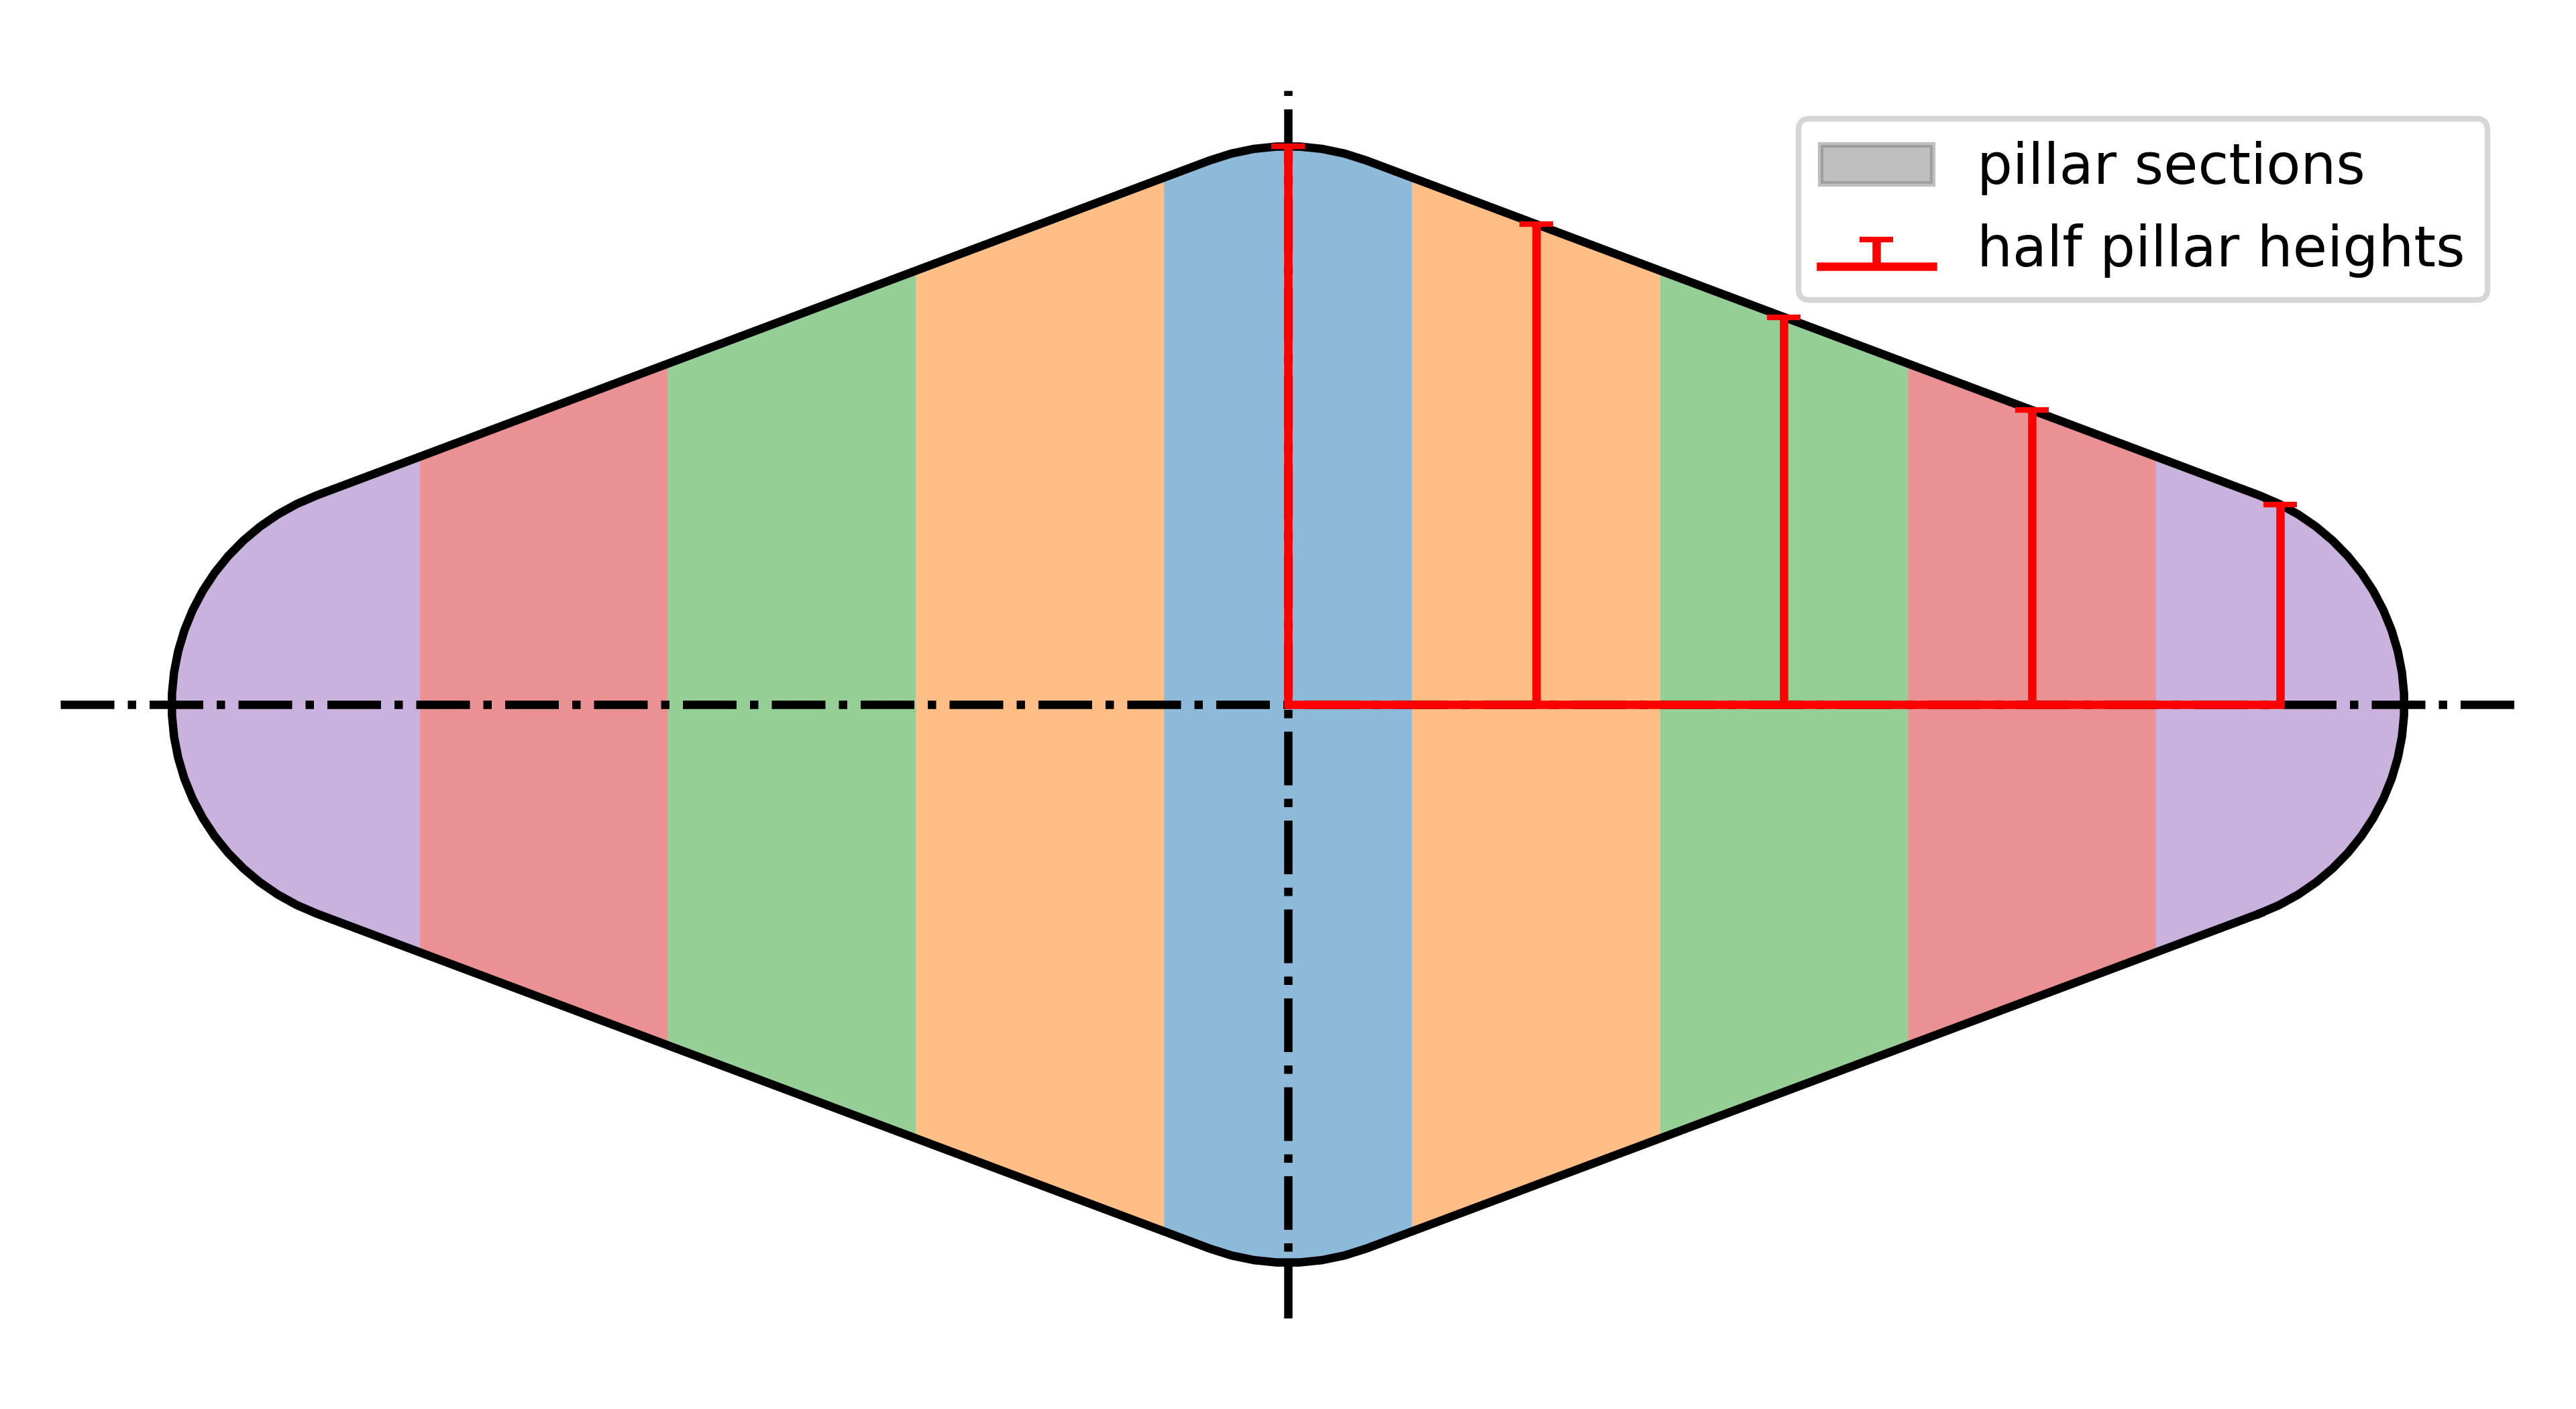
\includegraphics[width=0.6\linewidth]{img/pillar_profile}
        \caption{Example of Pillar Discretization for a Diamond Profile With 5 Pillars (Symmetrical)}
        \label{fig:pillar_profile}
    \end{figure}

    The pillar model introduces a discretization of the profile cross-section into distinct pillars as shown in \autoref{fig:pillar_profile}.
    The pillars' positions are defined by their center points $z_i$.
    $i \in [0, n - 1]$ is the index of the pillar, with $n$ as the count of pillars.
    Each pillar has a defined width $w_i$ and height $h_i$.
    The height is always measured at $z_i$.

    \begin{figure}
        \centering
        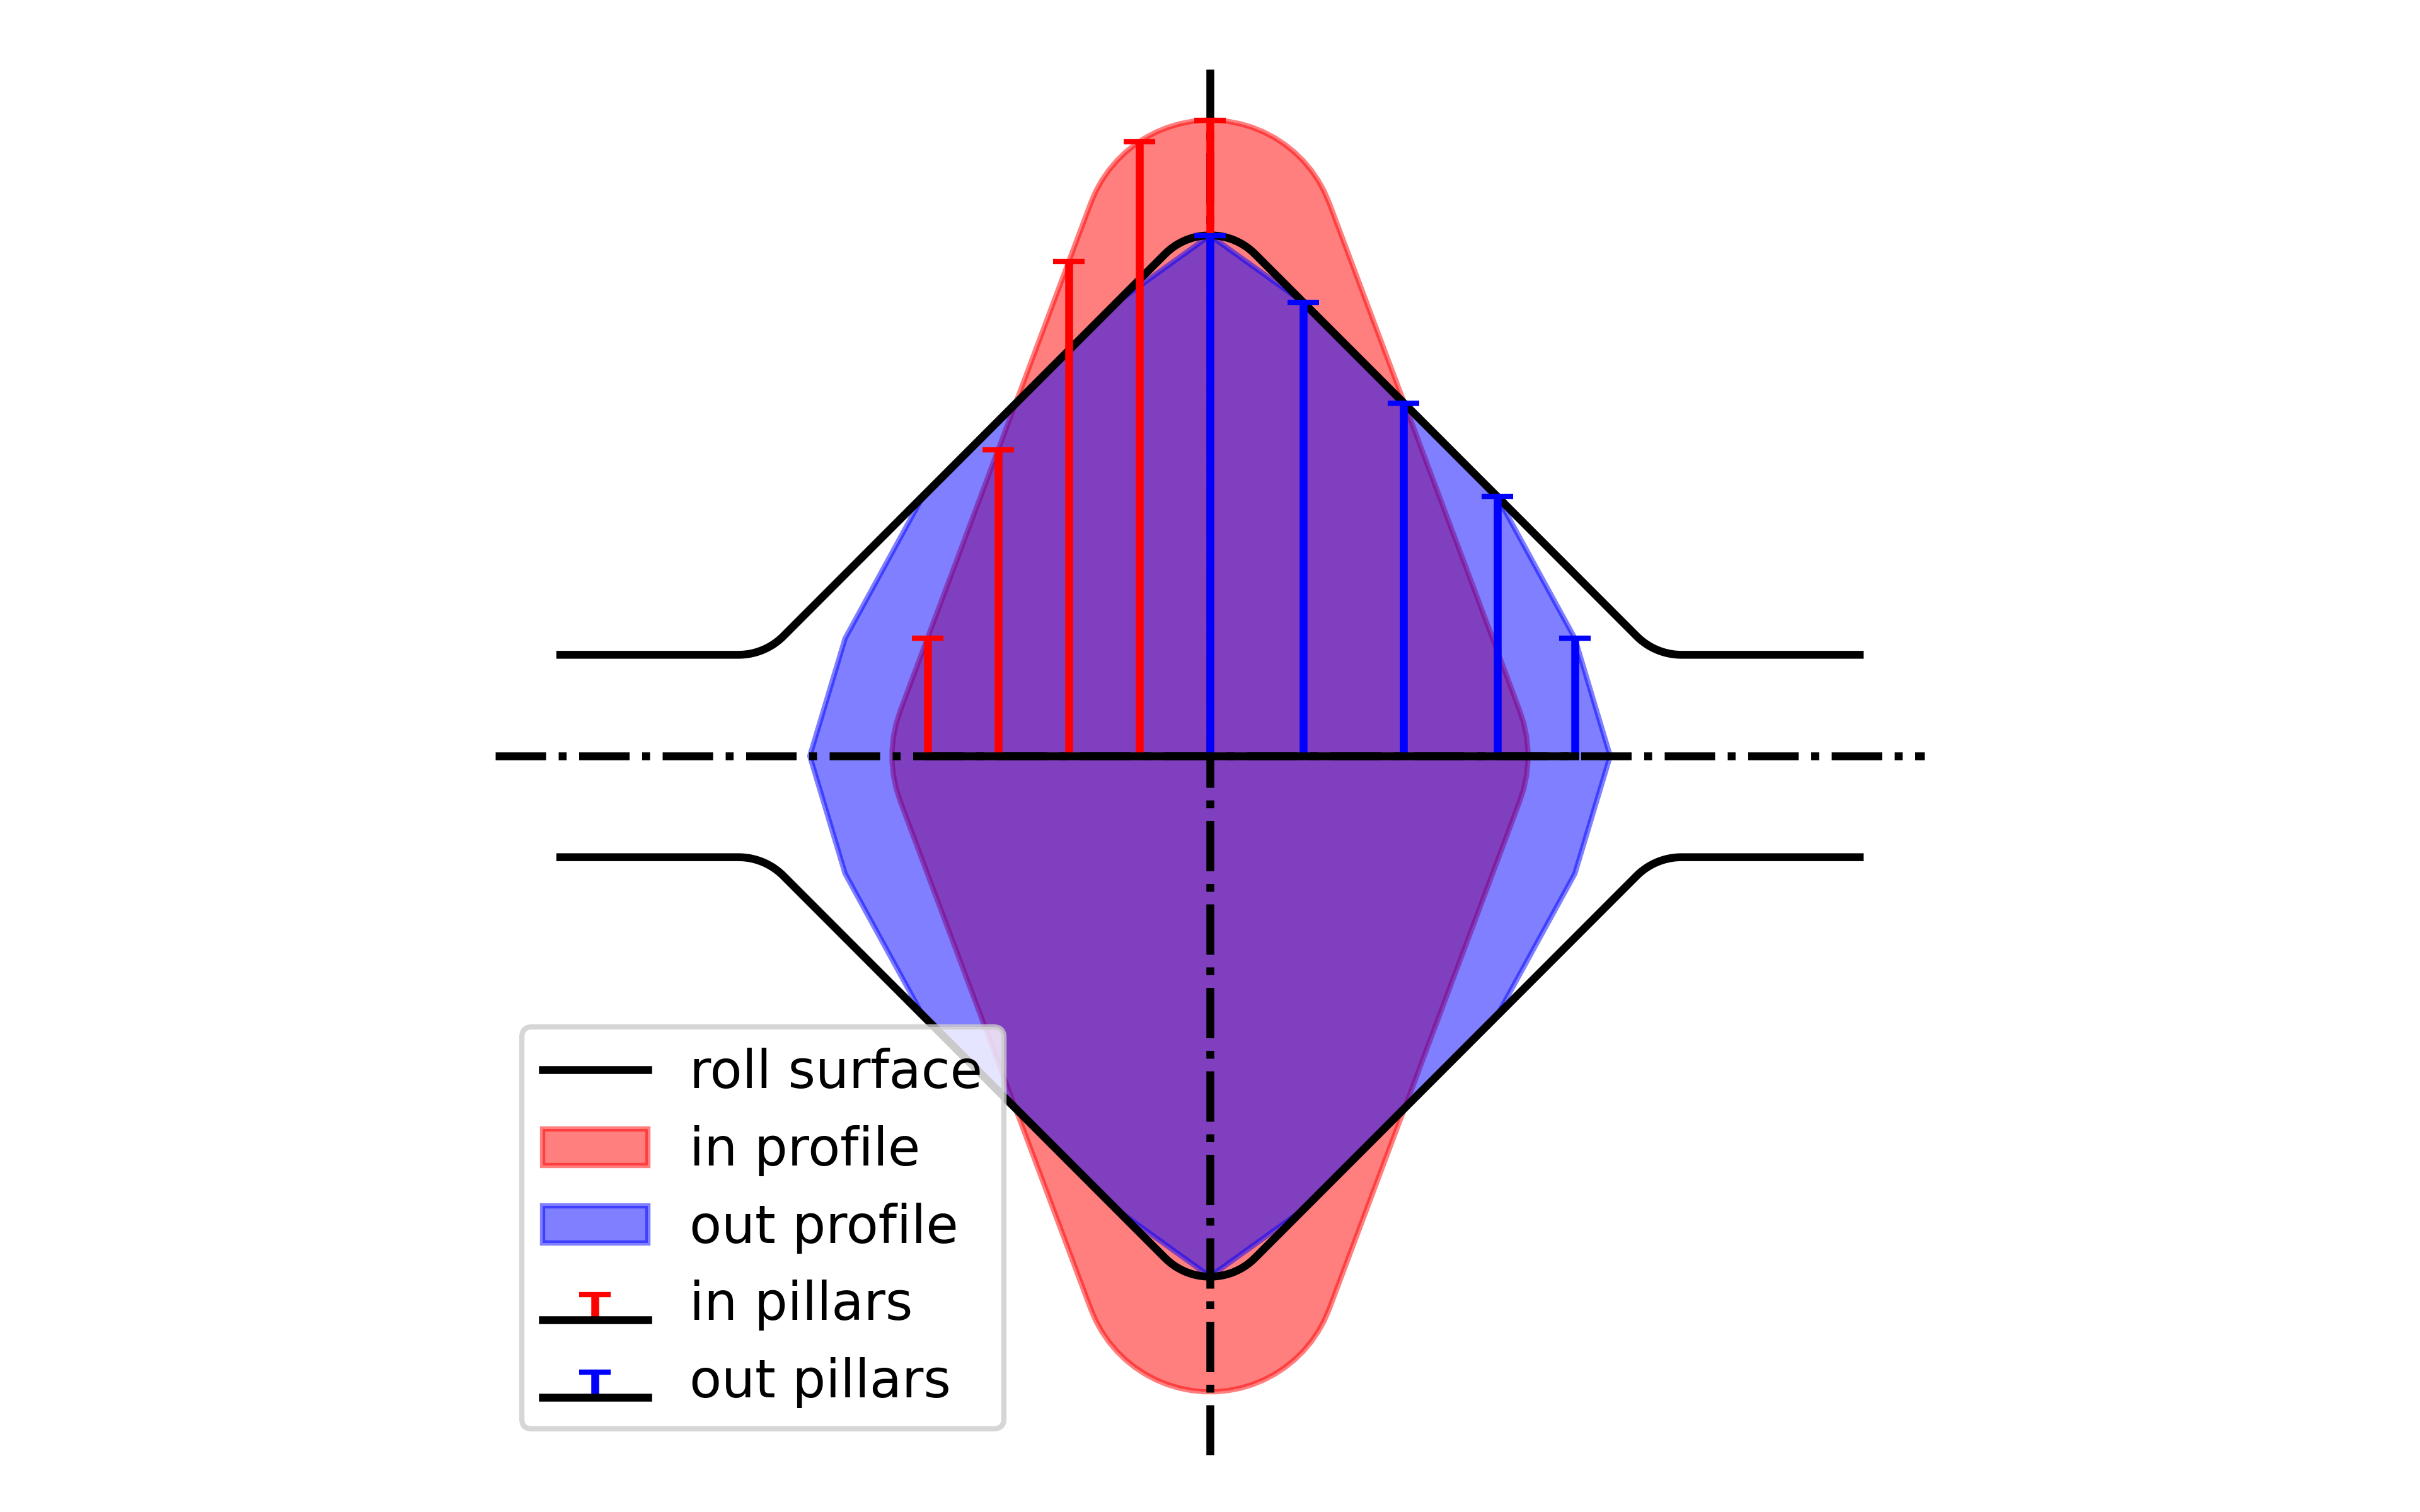
\includegraphics[width=0.6\linewidth]{img/pillar_disk_element}
        \caption{Deformation of a Pillared Profile in a Disk Element of a Roll Pass}
        \label{fig:pillar_disk_element}
    \end{figure}

    \autoref{fig:pillar_disk_element} shows the intended deformation of a pillar-discretized profile within a roll pass disk element.
    The incoming profile shows here a smooth surface, as it was generated by \py/Profile.diamond()/, the same way as the profile in \autoref{fig:pillar_profile}.
    The outgoing profile has lost its smooth surface, since the cross-section shape can only be described by the use of the pillars positions $z_i$ and heights $h_i$, so the cross-section becomes a linear line string.
    Note, that only the pillars 1--3 (from center to side) are here in contact with the roll surface, as their height is larger than the local roll pass height.
    Only they are experiencing deformation, with reduction in height and increase in width.
    The other pillars are shifted to the outside according to the others' widths, but maintain their heights.

    When discretizing an existing profile, the $z_i$ are calculated as in \autoref{eq:pillars}, with $w$ as the maximum profile width.
    However, during deformation the positions may change, so one shall not depend on equidistant pillars.

    \begin{subequations}
        \begin{gather}
            z_i = i \Delta z \\
            \Delta z = \frac{w}{n - \frac{1}{2}}
        \end{gather}
        \label{eq:pillars}
    \end{subequations}

    The boundaries $Z_j$ with $j \in [0, n]$ of the pillars are located halfway between their positions, but the innermost boundary is identical with the position $z_0 = Z_0 = 0$.

    \begin{equation}
        Z_j = \frac{z_j - z_{j-1}}{2}
        \label{eq:pillar_boundaries}
    \end{equation}

    The pillar widths $w_i$ are defined as the distance between their boundaries.
    Note, that the numerical width of the inner pillar $w_0$ is initially the half of the others due to $z_0 = Z_0 = 0$.

    \begin{equation}
        w_i = Z_{i+1} - Z_i
        \label{eq:pillar_widths}
    \end{equation}


    \section{Usage instructions}\label{sec:usage-instructions}

    Packages residing on this type of discretization shall depend on this plugin to create a common interface.
    In the following, the hooks defined by this plugin shall be described, and instructions shall be given, how to implement model equation for specific purposes.

    The ring model plugin only defines hooks on \py/pyroll.core.Profile/.
    The central hook of this package is \py/Profile.rings/.
    It returns a numpy array of radius coordinates representing the centers of the rings acc.\ to \autoref{eq:ring_center}.
    The respective ring boundaries' coordinates acc.\ to \autoref{eq:ring_boundaries}  are provided by the \py/Profile.ring_boundaries/ hook.
    The outermost boundary equals the equivalent radius acc.\ to \autoref{eq:equivalent_radius}  of the profile cross-section, which is also available from the \py/Profile.equivalent_radius/ hook.
    To modify the calculation of the equivalent radius, provide a new implementation of the \py/Profile.equivalent_radius/ hook.
    To modify the ring distancing, both \py/Profile.rings/ and \py/Profile.ring_boundaries/ should be provided.
    Users of this plugin should not rely on equidistant rings, but calculate needed distances from the respective coordinates.

    For geometric calculations, also two hooks returning shapely geometry objects are provided.
    \py/Profile.ring_contours/ returns an array of \py/LineStrings/ representing the mapping of the ring boundaries on the real profile cross-section.
    The interface lengths $I_j$ can be obtained by using \py/Profile.ring_contours[j].length/.
    \py/Profile.ring_sections/ returns, however, an array of \py/Polygon/ objects representing the areas of the rings lying between those boundaries.
    The ring cross-sections $A_i$ can be obtained by using \py/Profile.ring_sections[i].area/.

    For implementing model equations, define a new hook \py/Profile.ring_*s/ which shall return an array of the same length as \py/Profile.rings/.
    The \texttt{*} shall be replaced with the property name you want to represent, pay respect to the plural form.
    Ideally a hook named accordingly exists on \py/Profile/ or is defined alongside, which returns a mean value of the inhomogeneous data.
    For example the core hook \py/Profile.temperature/ may be accompanied by \py/Profile.ring_temperatures/ to hold inhomogeneous temperature data.

    \printbibliography

\end{document}